\section{Discussions}\label{sec:discuss}
% 
This section compares \xxx and \dare's protocols (\S\ref{sec:compare}), and 
discusses \xxx's limitations (\S\ref{sec:limits}) and its broad application 
areas (\S\ref{sec:apps}).

\subsection{Comparing \xxx and \dare}\label{sec:compare}

\begin{figure}[t]
\centering
\vspace{-.5in}
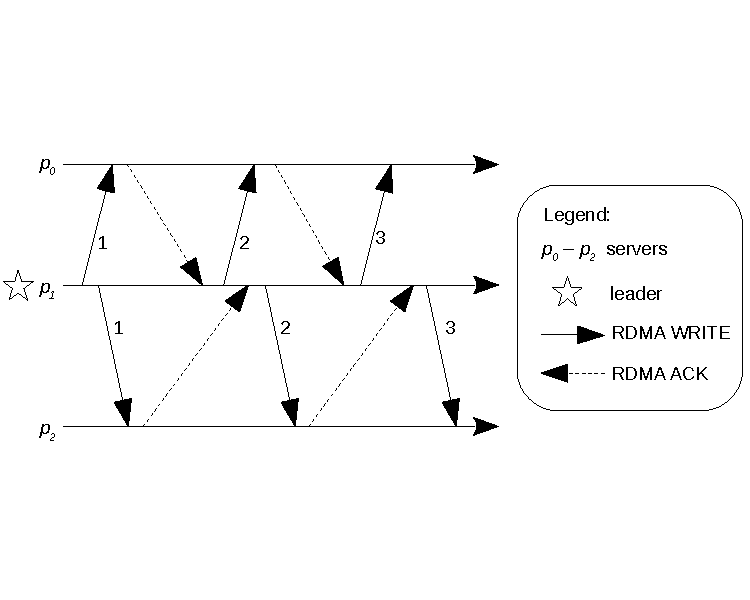
\includegraphics[width=.35\textwidth]{figures/dare}
\vspace{-.6in}
\caption{{\em \dare's RDMA-based consensus protocol.}} 
\label{fig:dare}
\vspace{-.20in}
\end{figure}

We highly appreciate \dare~\cite{dare:hpdc15}, the first RDMA-based, 
\paxos-like protocol. It is designed to run with a few replicas to tolerate 
single point of program failures. Therefore, \dare is most relevant to \xxx. 
Figure~\ref{fig:dare} shows \dare's consensus protocol in normal case. It is a 
sole-leader protocol (backups do not participate in consensus) with two rounds. 
In the first round, the leader uses RDMA to write the consensus requests to all 
replicas and polls RDMA ACKs to check whether the writes succeed. Second, for 
the successful writes, the leader does another round of RDMA writes to mark the 
writes as successful on other replicas, and poll ACKs on these writes. Once a 
majority of successful writes in the second round, DARE reaches a consensus.

\dare is well optimized for low latency with two technical choices. First, to 
avoid delays caused by polling ACKs, \dare uses a global RDMA CQ (Completion 
Queue) for all replicas, making it possible to collect multiple ACKs each poll 
operation. Second, this protocol does not incorporate a persistent storage or 
checkpoint/restore design. Therefore, \dare lacks durability 
(\S\ref{sec:background}), an important guarantee in \paxos practice. With these 
two choices, \dare runs slightly faster than \xxx on three replicas.

Unlike \xxx, \dare is not designed for high scalability. Our evaluation shows 
that, despite these two technical choices, both \dare's ACK pollings and its 
two-round consensus incurred scalability bottle approximately linearly consensus 
latency: DARE's consensus latency increased by \darescalability as replica group 
size increased by 35x (\S\ref{evaluation}).

Overall, \xxx differs from \dare in three aspects. First, \xxx is a one-round 
protocol, while \dare has two rounds. To achieve one-round consensus, \xxx 
requires backups to poll from its local memory to agree on requests, so \xxx 
consumes more CPU than \dare. Second, \xxx has shown toscale well on 100+ nodes, 
while \dare did not discuss or evaluate scalability in their paper. Third, to 
ensure durability, \xxx's protocol includes a persistent storage.

\subsection{\xxx Limitations}\label{sec:limits}

% Input coordination protocol.

% Have not hooked time and rand(). Can use PMP approach. Not a problem for 
% evaluated apps. 
\xxx currently does not hook random functions such as \v{gettimeofday()} and 
\v{rand()} because these random results are often explicit and easy to examine 
from network outputs (\eg, a timestamp in the header of a reply). Existing 
approaches~\cite{eve:osdi12,paxos:practical} in \paxos protocols can also be 
leveraged to intercept these functions and make them produce same results among 
replicas.
% because our output checkers have not detected network output 
% divergence comming from these functions

% Output checking protocol.

% Clamav style.
\xxx's output checking protocol may have false positives or false negatives, 
because it is just designed to try to improve assurance on whether replicas run 
in sync. A server program running in \xxx may have false positive when it uses 
multiple threads to serve the same client connection and uses these threads to 
concurrently add outputs (\eg, \clamav in our evaluation). 
Running a deterministic multithreading 
scheduler~\cite{coredet:asplos10,parrot:sosp13} with the server program 
addresses this problem.
% In our evaluation, all programs except \clamav uses only 
% one thread to process one client connection and they don't have such false 
% positives.

A server program may also have false negative when it triggers a software bug 
but the bug does not propagate to network outputs. From client programs' point 
of view, such bugs do not matter. Moreover, \xxx already checkpoints file 
system state to mitigate this issue.

Currently \xxx has not incorporated read-only optimization~\cite{eve:osdi12} 
because its performance overhead compared to the evaluated programs' 
unreplicated executions is already reasonable (\S\ref{sec:overhead}). However, 
\xxx can be extended to support read-only optimization if two conditions are 
met: (1) whether the semantic an operation is read-only is clear in a server 
program; and (2) the number of output bytes for this operation is fixed. GET 
requests in key-value stores often meet these two conditions.

We use GET requests to present a design. \xxx intercepts a client program's 
outbound socket calls (\eg, \send), compares the first three bytes in each call 
with ``GET". If they match, \xxx appends two extra \xxx metadata fields 
\v{read\_only} and \v{length} in this outbound call to the server. \xxx then 
intercepts a server's \recv calls and strips these two fields. If the first 
field is true, \xxx directly processes this operation in a local replica 
and strips the next \v{length} bytes from the output checker within the same
connection. In sum, \xxx processes these operations locally without making 
outputs across replicas diverge.

% When execution divergence is detected in a replica, \xxx's rollback mechanism 
% is not designed to guarantee that the re-executions of this replica will 
% definitely avoids this divergence. We made this design choice because both 
% our evaluation and a previous work Eve~\cite{eve:osdi12} found that divergence 
% happens extremely rarely in evaluation. In our evaluation, we found that simply 
% re-executing the log can practically make \xxx's replicas converge to 
% same execution states. A similar finding is that although Eve provided a 
% sequential re-execution approach to with divergence avoidance guarantee, which 
% \xxx can leverage, but even Eve's evaluation didn't experience any divergence 
% and thus this approach was not invoked.

% Read only opt?

% No guarantees on recovery. Best effort. But, can we actually server requests 
% one by one?

%% No lxc.

%% Support for Java may not be good due to the VM memory copying. Some 
% techniques that avoid memory copying may be usable~\cite{weixu:tsinghua}. Good 
% for % C/C++ programs as long as they use POSIX socket APIs.



\subsection{\xxx Has Broad Applications}\label{sec:apps}

In addition to greatly improving the availability of general server programs, 
we envision that \xxx can be applied in broad areas, and here we elaborate 
three. First, \xxx's RDMA-accelerated \paxos protocol and its implementation 
could be a template for other replication protocols (\eg, byzantine 
fault-tolerance~\cite{zyzzyva:sosp07,pbft:osdi99}). 

% Another promising direction is three-phase commit (3PC): 3PC is often 
% blamed by its intolerance on network partitions and asynchronour 
% communications, 
% and its high latency caused by the three round-trips. Fortunately, within the 
% RDMA-enabled datacenter context, people may leverage \xxx's techniques and 
% experience to build a significantly faster and more reliable 3PC protocols.

% Other replication topics.

% Parallel program analysis. Such a short coordination time can make replicas 
% run almost as fast as each other, support many time-critical analyses 
% such as race detection and security defenses.
Second, by efficiently constructing multiple, equivalent executions for the 
same program, \xxx can benefit distributed program analysis techniques. Bounded 
by the limited computing resources on single machine, recent advanced 
program analysis frameworks become 
distributed~\cite{decouple:usenix08, speck:asplos08, 
shadowreplica:ccs13, wester:parallelizing:asplos13,repframe:apsys15} in order to 
offload analyses on multiple machines. \xxx can be leveraged in these 
frameworks so that developers of analysis tools can just focus on their own 
analysis logic, while \xxx's general replication architecture handles the rest.

Moreover, program analyses developers can tightly integrate their tools with 
\xxx. For instance, they can proactively diversify the orders of socket calls 
in \xxx's consensus logs among replicas to improve replicas' tolerance on 
security attacks~\cite{con:hotpar12}.

% TBD: use \xxx to detect software bugs by checking outputs, even in 
% real-world deployments. XXX make program % inputs strongly consistent across 
% replicas, so output divergence are likely % from software bugs. XXX promising 
% 
% results in our evaluation. Find a bug in % ssdb?

% One idea: can leverage the checkpoint and rollback protocok, and the 
% consensus part, to build a system that can automatically bypass concurrency 
% bugs without fixing them. The way to bypass: proactively reordering socket 
% calls. Self-healing system.

% A core building block in future operating systems. Maintain a consistent view 
% of computing resources and data. Used in scheduling framework (Mesos) because 
% its latency is almost compatible with context switches of processes (sub 
% milli seconds).
Third, \xxx can be a core building block in the emerging datacenter operating 
systems~\cite{matei:hotcloud11, mesos:nsdi11, datacenter:os}. As a 
datacenter continuously emerges a computer, an OS may be increasingly needed for 
such a giant computer. \xxx's fast, general coordination service is especially 
suitable for such an OS's scheduler to maintain a consistent, reliable view on 
both computing resources and data in a datacenter. For instance, \xxx's 
latency is largely between less than 30 \us, much smaller than a typical 
process context switch (a few hundreds \us).
